\section{熱化学平衡における分子混合率}

系外惑星大気中の分子の存在量は、高温高圧の場合は熱化学平衡に近づくと考えられる。鉛直輸送や光化学反応、もしくは低温系大気の場合あっても、熱化学平衡の時にどうなるかは一つの基準として知っておくべきである。
そこで、ここでは熱化学平衡に至っている場合の大気中の分子中の混合率がどのように決定されるか考える。\\

\subsection*{元素の保存}

ガス中には\ce{H2}や\ce{H}、\ce{H2O}をいった分子種や原子種、イオン、自由電子が適当な割合で混合している。これらをまとめて{\bf 種}(species)と呼ぶ。これら大気種中に含まれる原子の総数を考えたい。ガス中に含まれる種の中の原子(例えば\ce{H, O, C})ではなく、ガス中のすべての分子や原子に含まれる原子を{\bf 元素}(elements)と呼び区別する。本文書では元素をサンセリフ体を用いて、$\Hel$, $\Oel$, $\Cel$のようにあらわす。\\

\subsection*{二成分系の場合}

まず最も単純な以下の水素原子と水素分子のガス2成分系
\begin{align*}
\ce{2 H <--> H2}
\end{align*}
の場合、熱化学平衡でどのような組成比になるかを考えてみよう\footnote{実際は少量の触媒Mを介して\ce{2 H + M <--> H2 + M}としたほうが現実的だが、ここでは数学的側面を重視しMを無視する。}。この場合、種は\ce{H}と\ce{H2}の二種類($N_s = 2$)であり、元素は$\Hel$の一種類($N_e = 1$)である。

いま元素量として$\nel_{\Hel}$(例えば1 mol)の水素を考える。すなわち元素保存則は
\begin{align}
    n_\mathrm{H} + 2 n_\mathrm{H2}  = \nel_{\Hel} 
\end{align}
となる。圧力$P$と温度$T$を与えたときに、熱化学平衡条件を満たす場合に、この元素$\Hel$がどのように\ce{H}と\ce{H2}に分配されるかを与えるのが、ギブス自由エネルギーの最小化である。すなわち熱化学平衡においては種の存在量は以下の最小化で与えられる
\begin{align}
\label{eq:opt1tce}
    &(n_\mathrm{H}^\ast, n_\mathrm{H2}^\ast) = \mathrm{minimize}_{(n_\mathrm{H}, n_\mathrm{H2})} \,\, G(T, P, n_\mathrm{H}, n_\mathrm{H2}) \,\, \\ 
    &\mbox{subject to} \,\, n_\mathrm{H} + 2 n_\mathrm{H2} =  \nel_{\Hel}  \\
    &G(T, P, n_\mathrm{H}, n_\mathrm{H2}) = n_\mathrm{H} \mu_\mathrm{H} + n_\mathrm{H2} \mu_\mathrm{H2} \\
     &\, n_\mathrm{H} \ge 0, n_\mathrm{H2} \ge 0
\end{align}
ここに$\mu_\mathrm{H}$、$ \mu_\mathrm{H2}$は\ce{H}, \ce{H2}の化学ポテンシャルであり、標準状態の化学ポテンシャルを用いると
\begin{align}
    \mu_\mathrm{H} &= \mu_\mathrm{H}^o(T) + RT \log{\frac{P_\mathrm{H}}{P_\mathrm{ref}}} \\
    &=  \mu_\mathrm{H}^o(T) + RT \log{\frac{n_\mathrm{H} P}{(n_\mathrm{H} + n_\mathrm{H2}) P_\mathrm{ref}}} \\
    \mu_\mathrm{H2} &= \mu_\mathrm{H2}^o(T) + RT \log{\frac{P_\mathrm{H2}}{P_\mathrm{ref}}} \\
    &=  \mu_\mathrm{H2}^o(T) + RT\log{\frac{n_\mathrm{H2} P}{(n_\mathrm{H} + n_\mathrm{H2}) P_\mathrm{ref}}}
\end{align}
で与えられる。$\partial G/\partial n_\mathrm{H} = \mu_\mathrm{H}$, $\partial G/\partial n_\mathrm{H2} = \mu_\mathrm{H2}$が満たされることを確認せよ。

ここでは後の一般化を考え、上の等式条件付き最適化をラグランジュ未定乗数法で解く。ラグランジュ未定乗数法では、自由パラメタを$\xv = ( n_\mathrm{H},  n_\mathrm{H2}, \lambda )^\top$の3パラメタとして
\begin{align}
\label{eq:opt2tce}
    \xv_\ast &= \mathrm{minimize}_{\xv} \,\, \mathcal{L} (T, P, \xv) \\ 
    \mathcal{L} (T, P, \xv) &\equiv G(T, P, \xv) + \lambda (n_\mathrm{H}  + 2 n_\mathrm{H2} - \nel_{\Hel} ) \\
    \label{eq:nonnegative_tce}
    &n_\mathrm{H} \ge 0, n_\mathrm{H2} \ge 0
\end{align}
を解けばよい。最後の非負条件は後でチェックする。$\mathcal{L} (T, P, \xv)$を$\xv$で偏微分したものが$\boldsymbol{0}$であるとして、$\xv=\xv_\ast$を求める。すなわち
\begin{align}
&\frac{\partial \mathcal{L} (T, P, \xv)}{\partial \xv} = 
\begin{pmatrix}
    \mu_\mathrm{H} + \lambda \\
    \mu_\mathrm{H2} + 2 \lambda \\
    n_\mathrm{H} + 2 n_\mathrm{H2} -  \nel_{\Hel} 
\end{pmatrix}\\
&=
\displaystyle{
\begin{pmatrix}
    \mu_\mathrm{H}^o(T) + RT \log{\frac{n_\mathrm{H} P}{(n_\mathrm{H} + n_\mathrm{H2}) P_\mathrm{ref}}}  + \lambda \\
    \mu_\mathrm{H2}^o(T) + RT\log{\frac{n_\mathrm{H2} P}{(n_\mathrm{H} + n_\mathrm{H2}) P_\mathrm{ref}}} + 2 \lambda \\
    n_\mathrm{H} + 2 n_\mathrm{H2} -  \nel_{\Hel} 
\end{pmatrix}
}
=
\begin{pmatrix}
    0 \\
    0 \\
    0
\end{pmatrix}
\end{align}
である。第1,2成分から$\lambda$について消去すると
\begin{align}
    \log{\left( \frac{n_\mathrm{H}^2 }{n_\mathrm{H2} (n_\mathrm{H} + n_\mathrm{H2})} \frac{P}{P_\mathrm{ref}} \right)} =- \frac{2 \mu_\mathrm{H}^o - \mu_\mathrm{H2}^o}{RT} 
\end{align}
がえられる。第3成分(保存則)$n_\mathrm{H} + 2 n_\mathrm{H2} - \nel_{\Hel}=0$をもちいて、$n_\mathrm{H2}$を消去すると、
\begin{align}
\frac{ \nel_{\Hel}^2 - n_\mathrm{H}^2}{4 n_\mathrm{H}^2} = \frac{P}{P_\mathrm{ref}} 
\exp{\left( - \frac{\mu_\mathrm{H2}^o - 2 \mu_\mathrm{H}^o}{RT} \right)}  \equiv k
\end{align}
であり、$n_\mathrm{H} \ge 0$より
\begin{align}
 \frac{n_\mathrm{H}}{ \nel_{\Hel} } = \frac{1}{\sqrt{4 k + 1}}
\end{align}
また保存則より
\begin{align}
 \frac{n_\mathrm{H2}}{ \nel_{\Hel} } = \frac{1}{2} \left( 1 - \frac{1}{\sqrt{4 k + 1}} \right)
\end{align}
となる。これらは水素元素$\nel_{\Hel}$あたりの分子量となっていることに注意する。つまり実務上は$\nel_{\Hel}=1$ (mol)ととって計算を進めてもよい。

また体積分率(Volume Mixing Ratio)は
\begin{align}
 \mathrm{VMR} (\ce{H}) &= \frac{n_\mathrm{H}}{n_\mathrm{tot}} = \frac{1}{2} \left( \sqrt{k^2 + 4 k} - k \right) \\
  \mathrm{VMR} (\ce{H2}) &= \frac{n_\mathrm{H2}}{n_\mathrm{tot}} = \frac{1}{2} \left( 2 + k - \sqrt{k^2 + 4 k}\right)
\end{align}
となる。図\ref{fig:temperature_exogibbs}に混合率の温度依存性を図示した。

\begin{figure}
    \centering
    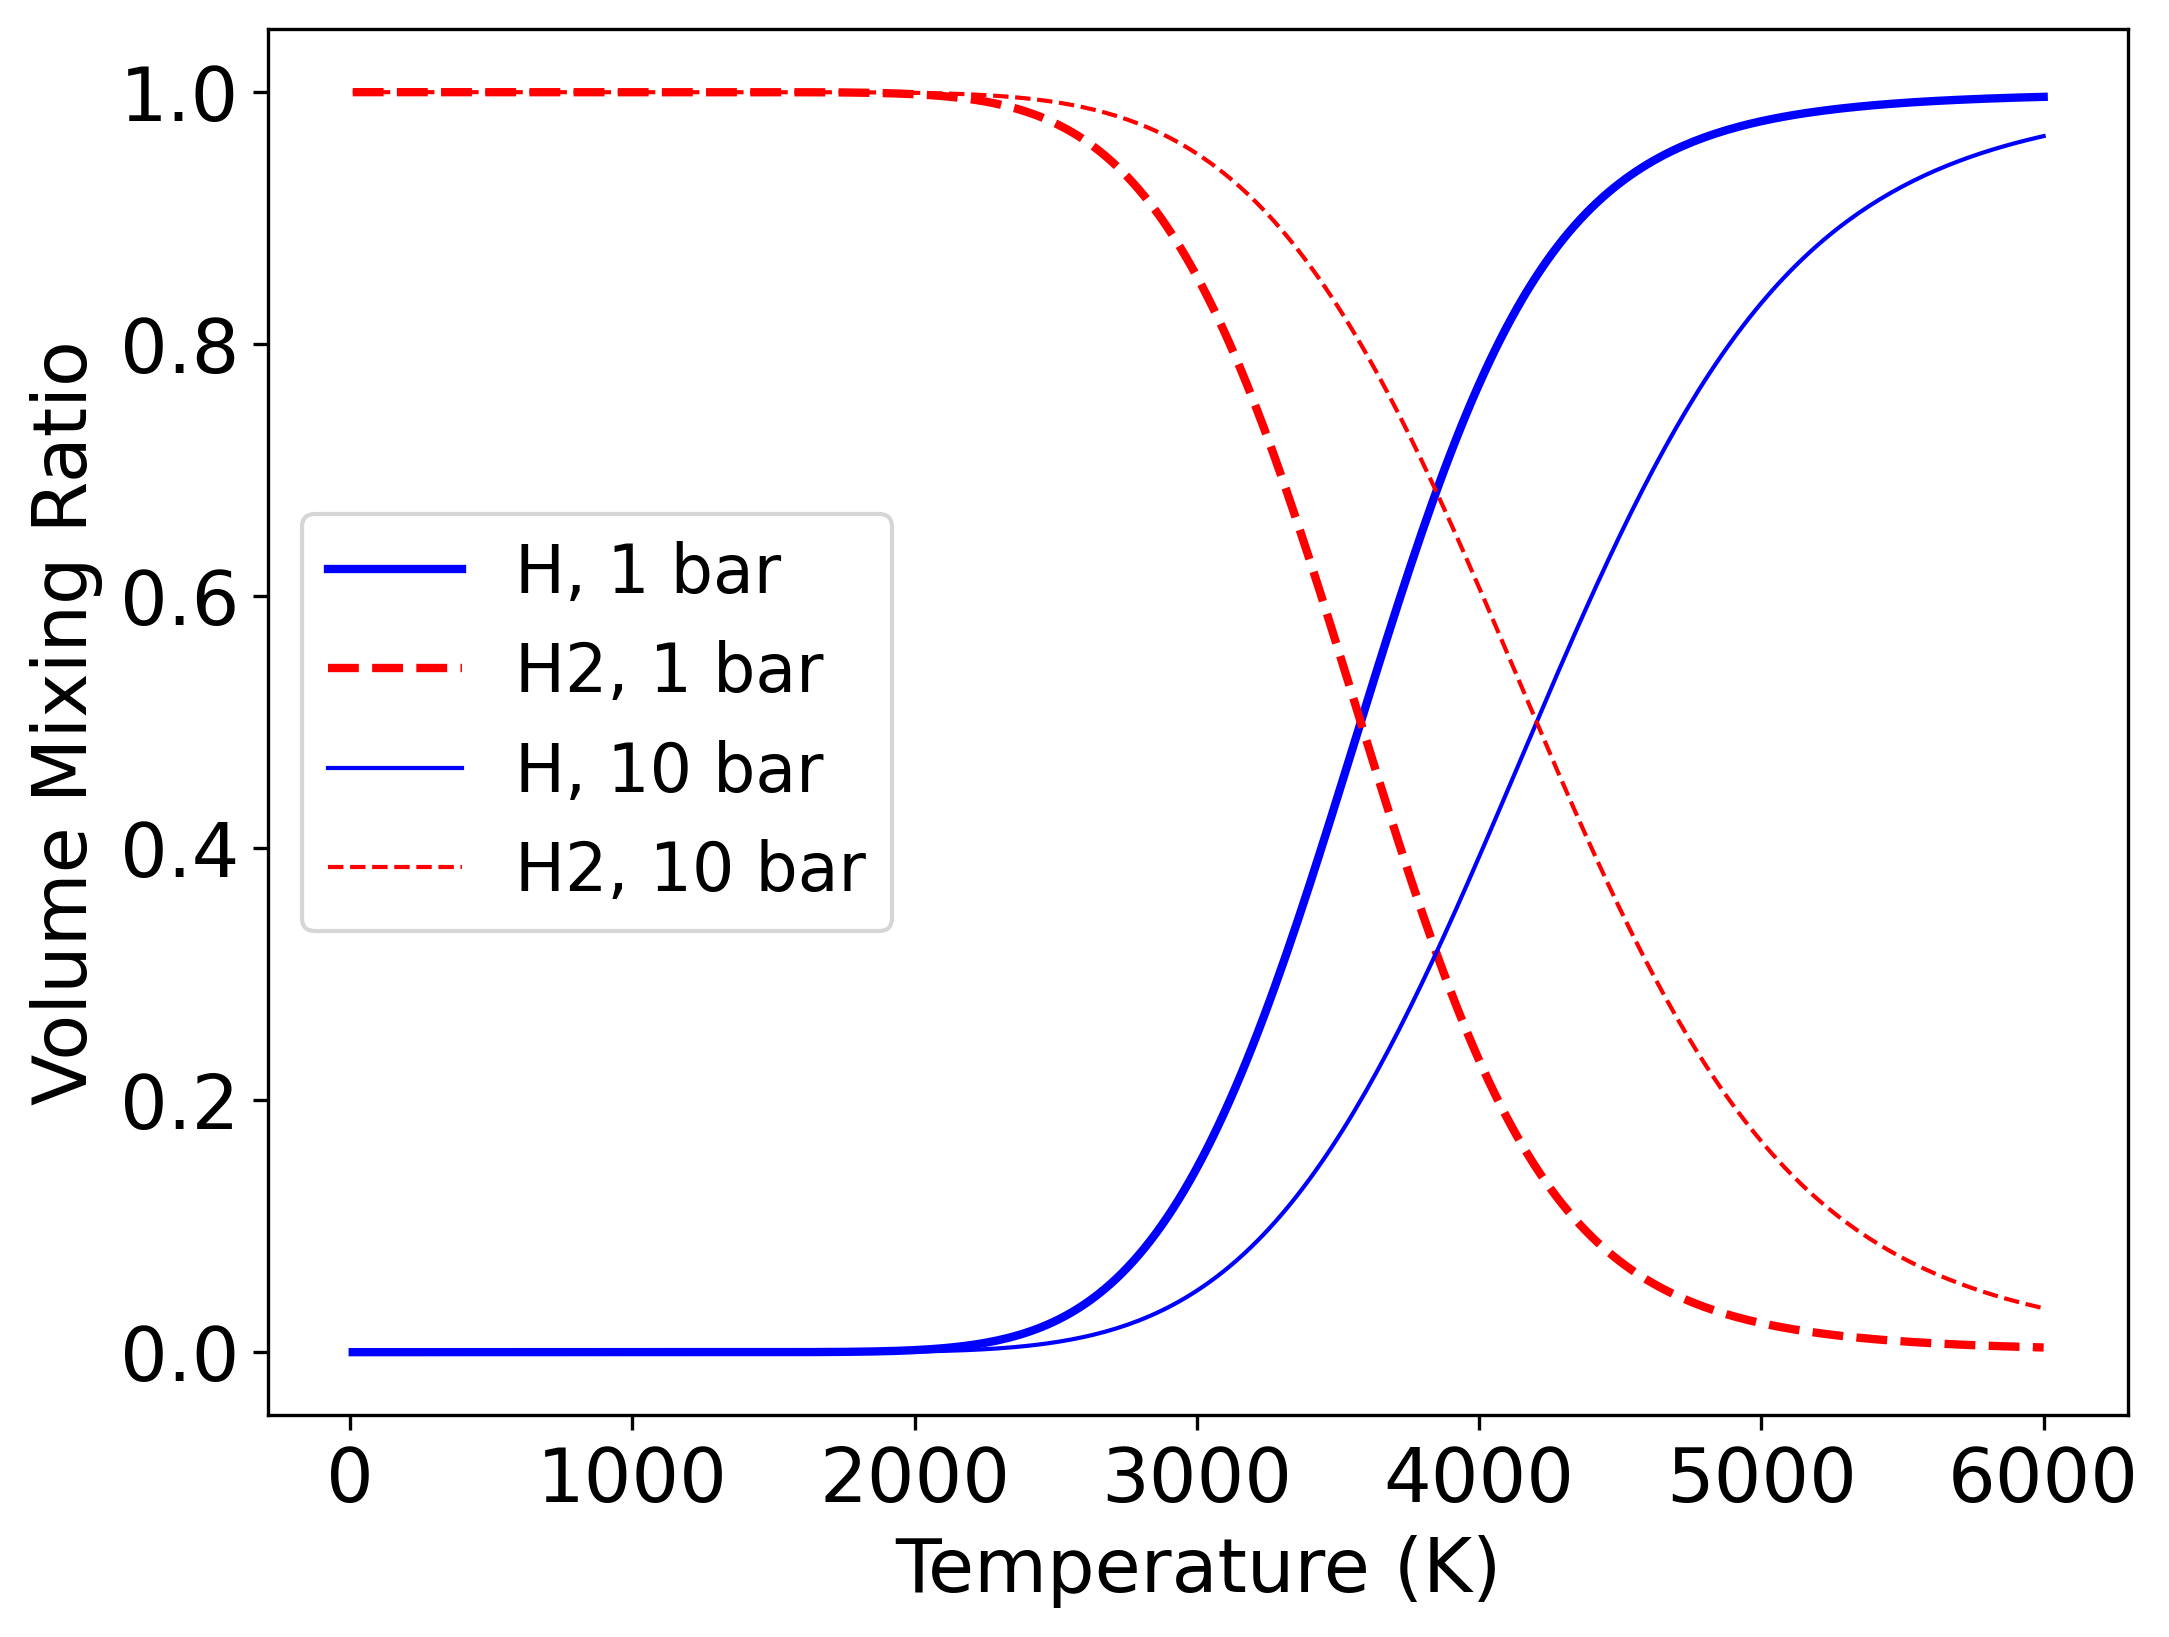
\includegraphics[width=\linewidth]{fig/tce_two_species.png}
    \caption{\ce{2 H <--> H2}の熱化学平衡の体積混合率}
    \label{fig:temperature_exogibbs}
\end{figure}

\subsection*{多成分系の場合$^\ddagger$}

次に多元素系を考える. 
今,例として元素として$\Hel, \Cel, \Oel$,また種としては\ce{CO, H2, CH4, H2O}からなる系を考えよう. これらは水素大気の分子成分としては主要なものである. 化学反応としては以下の一つの反応式となる. 
\begin{align*}
\ce{CO + 3 H2 <--> CH4 + H2O}
\end{align*}
となる. 


要素との化学反応式を考えると,
\begin{align*}
\ce{H2 <--> 2 $\Hel$ \, \, \, \, \, \, \, \, \\
H2O <--> 2 $\Hel$ + 1 $\Oel$ \\
CH4 <--> 4 $\Hel$ + 1 $\Cel$ \\
CO <-->  1 $\Cel$ + 1 $\Oel$
}
\end{align*}
のようになる. ここで,0成分も含んで表現すると
\begin{align*}
\ce{H2 <--> 2 $\Hel$ + 0 $\Cel$ + 0 $\Oel$ \\
H2O <--> 2 $\Hel$ + 0 $\Cel$ + 1 $\Oel$ \\
CH4 <--> 4 $\Hel$ + 1 $\Cel$ + 0 $\Oel$ \\
CO <--> 0 $\Hel$ + 1 $\Cel$ + 1 $\Oel$ \\ 
}
\end{align*}
のようになる. 右辺についてformula matrixを以下のように定義する. 
\begin{align*}
  A \equiv
\begin{pmatrix} 
2 & 2 & 4 & 0 \\
0 & 0 & 1 & 1 \\
0 & 1 & 0 & 1 
\end{pmatrix}  
\end{align*}

種の存在量ベクトルを$\nv = (n_\mathrm{H_2}, n_\mathrm{H_2 O},n_\mathrm{C H_4},n_\mathrm{CO})^\top$,元素の存在量ベクトルを$\bv = (\nel_\Hel, \nel_\Cel, \nel_\Oel)^\top$と置くと(元素の存在量を種とは区別している点に注意),元素保存則は
\begin{align}
    A \, \nv = \bv 
\end{align}
と表されることが分かる. 


多元素系でも同様に,以下のGibbsエネルギーを最小化すればよい
\begin{align}
\label{eq:gibss_multi}
    \nv^\ast &= \mathrm{minimize}_{\nv} G(T, p, \nv) \nonumber \\
    &\mbox{subject to} \,\, A \, \nv = \bv, n_i \ge 0\\
    G(T, p, \nv) &\equiv  \muv (T, P, \nv)^\top \nv\\ 
    \label{eq:chemical_potential_mu}
    \muv (T, p, \nv) &=  \muv^\circ(T) + RT \log{\left(\frac{p}{\ntot} \nv\right)} 
\end{align}
ただし総数密度と規格化圧力を
\begin{align}
\label{eq:ntot_tce}
    \ntot &= \sum_i n_i \\
    p &\equiv P/P_\mathrm{ref}
\end{align}
と定義した. 

\ce{CO, H2, CH4, H2O}系において, 式(\ref{eq:gibss_multi})は,
\begin{align}
    \mathcal{L}(T, p, \nv,\lambdav) &= \sum_{i = \ce{CO, H2, CH4, H2O}} \mu_i (T) \, n_i \nonumber \\ &+ \lambda_{\Hel} (2 n_{\ce{H2}} + 4 n_{\ce{CH4}} + 2 n_{\ce{H2O}} - b_\Hel) \nonumber \\
    &+ \lambda_{\Cel} (n_{\ce{CO}} + n_{\ce{CH4}} - b_\Cel) \nonumber \\ 
    &+  \lambda_{\Oel} ( n_{\ce{CO}} + n_{\ce{H2O}} - b_\Oel)
\end{align}

ここではGordon and McBrideによるNASA/CEA (Chemical Equilibrium with Applications)の実装法を元に解説する\cite{gordon1994computer,2024arXiv241207166G}. CEAではLagrange multiplierを用いてGibbsエネルギー最小化を行う二次の手法の一つである. すなわち
\begin{align}
    (\nv^\ast, \lambdav)  &= \mathrm{minimize}_{(\nv,\lambdav)} \,\, \mathcal{L}(T, p, \nv, \lambdav) \\
    \mathcal{L}(T, p, \nv,\lambdav) &= G(T, p, \nv) + \lambdav^\top \left(A \nv - \bv\right)  
\end{align}
を最小化する. ただしこの時点では非負条件$n_i \ge 0$は外れていない. 

$\mathcal{L}(T, p, \nv, \lambdav)$の停留点を求めるために,最適化変数のセット$\yv = (\nv, \lambdav)$で一次偏微分した関数を
\begin{align}
\label{eq:fv_tea0}
    \fv(\yv) &\equiv \frac{\partial  }{\partial \yv} \mathcal{L}(T, p, \yv) 
\end{align}
を定義する. そして
\begin{align}
    \label{eq:fv_tea}
    \fv(\yv^\ast) = \boldsymbol{0}
\end{align}
の解をNewton法でもとめることで,$\yv^\ast = (\nv^\ast, \lambdav^\ast)$を求める. 次に式(\ref{eq:fv_tea0})の$\nv$成分を計算する
\begin{align}
\label{eq:Lpartialn}
    \frac{\partial}{\partial \nv}   \mathcal{L}(T, p, \nv, \lambdav) =  \muv (T, P, \nv) + A^\top \lambdav  
\end{align}
ここに熱力学より$\partial_{\nv} G(T, p, \nv) =  \muv (T, P, \nv)$\footnote{式(\ref{eq:chemical_potential_mu})を用いて直接確かめることができる. }および$\lambdav^\top (A \nv) = (A^\top \lambdav)^\top \nv$と$\partial_{\xv} (S^\top \xv) = S$を利用した. 
式(\ref{eq:Lpartialn})は$\lambdav$について一次である点に注意する. $\lambdav$成分は単に保存関係
\begin{align}
\label{eq:Lpartiall}
\frac{\partial}{\partial \lambdav}  \mathcal{L}(T, p, \nv, \lambdav) = A \nv - \bv  
\end{align}
である. 

式(\ref{eq:chemical_potential_mu})を用いるとNewton法で解くべき方程式系(\ref{eq:fv_tea})は
\begin{align}
\label{eq:Lpartialnx}
    \frac{\muv^\circ(T)}{RT}+ \log{\left(\frac{p}{\ntot^\ast} \nv^\ast \right)} + \frac{A^\top \lambdav^\ast}{RT}   &= \boldsymbol{0} \\
    A \nv^\ast - \bv &= \boldsymbol{0}
\end{align}
となる. ただし$\ntot^\ast$は$\nv^\ast$の関数,すなわち
\begin{align}
\ntot^\ast &= \sum_i n_i^\ast
\end{align}
となる. 


ここでCEAのアルゴリズムではいくつかのトリックを用いる. まず,式(\ref{eq:fv_tea})を求めるために,独立変数に$\ntot$を追加する. もともと$\ntot$は式(\ref{eq:ntot_tce})により$\nv$に依存していたため,この条件,つまり式(\ref{eq:ntot_tce})を,(前提条件ではなく)制約条件として追加する. さらに$\nv$, $\ntot$は対数を取ったものを独立変数に取り直す. つまり$\lnnv = \ln{\nv}$, $\lnntot = \ln{\ntot}$を独立変数とする.  この操作により非負条件$n_i \ge 0$は自然に取り除かれる. また対数を取ることで広いダイナミックレンジで安定し
た数値計算となる. これにより新たな変数系として$\zv = (\lnnv, \lambdav, \lnntot)$が導入され,解くべき方程式は
\begin{align}
\label{eq:Lpartialncea}
    \Fv_n (\zv) &\equiv \frac{\muv^\circ(T)}{RT} + \lnnv - \lnntot \, \uv + \log{p} \, \uv  + \frac{A^\top \lambdav}{RT}  \\
    \Fv_\lambda (\zv) &\equiv A e^{\lnnv} - \bv = \boldsymbol{0}_M \\
    F_\mathrm{tot} (\zv) &\equiv \sum_i {e^{q_i}} - e^{\lnntot} = 0
\end{align}
の解
\begin{align}
  \Fv_n (\zv) &= \boldsymbol{0}_M \\
  \Fv_\lambda (\zv) &= \boldsymbol{0}_M \\
  F_\mathrm{tot} (\zv) &= 0
\end{align}
である. $\boldsymbol{0}_M$は$M$次元ゼロベクトルである. この解が$\zv^\ast = (\lnnv^\ast, \lambdav^\ast, \lnntot^\ast)$となる. これを簡潔に$\Fv (\zv) = (\Fv_n (\zv), \Fv_\lambda (\zv), F_\mathrm{tot} (\zv))$とまとめて扱うこともある.  

Newton法では$\Fv (\zv)$を$\zv$で微分したヤコビアンが必要となる. 
\begin{align}
\label{eq:jacobian_tce}
\Jv (\zv) &=
\left(
\begin{array}{ccc}
    \dfrac{\partial \Fv_n}{\partial \lnnv}  & \dfrac{\partial \Fv_n}{\partial \lambdav}& \dfrac{\partial \Fv_n}{\partial \lnntot}\\ 
    \dfrac{\partial \Fv_\lambda}{\partial \lnnv} & \dfrac{\partial \Fv_\lambda}{\partial \lambdav} & \dfrac{\partial \Fv_\lambda}{\partial \lnntot} \\
    \dfrac{\partial F_\mathrm{tot}}{\partial \lnnv} & \dfrac{\partial F_\mathrm{tot}}{\partial \lambdav} & \dfrac{\partial F_\mathrm{tot}}{\partial \lnntot} \\  
\end{array}
\right) \nonumber \\
&=
\left(
\begin{array}{ccc}
 E_M &  \dfrac{A^\top}{RT} & - \uv\\ 
 Y(\lnnv) & Z_M & \boldsymbol{0}_M \\ 
 (e^{\qv})^\top & \boldsymbol{0}_M^\top & - e^\lnntot\\  
\end{array}
\right)
\end{align}
となる. ここに
$E_M$は$M \times M$単位行列,$Z_M$は$M \times M$ゼロ行列, $M$は元素ベクトル$\bv$の要素数である. また行列$Y(\lnnv)$は
$Y(\lnnv)= A \, \mathrm{diag}(e^{\lnnv}) $のことであり,すなわち要素が
\begin{align}
Y_{ij} = A_{ij} e^{q_j}
\end{align}
であるような行列である. Newton法のupdateは式(\ref{eq:second_newton})より,$\Jv (\zv_k) \Delta \zv = - \Fv (\zv_k)$をみたすので
\begin{align}
    \left(
\begin{array}{ccc}
 E_M &  \dfrac{A^\top}{RT} & - \uv\\ 
 Y(\lnnv) & Z_M & \boldsymbol{0}_M \\ 
 (e^{{\lnnv}_k})^\top & \boldsymbol{0}_M^\top & - e^{(\lnntot)_k}\\  
\end{array}
\right)
    &\left(
\begin{array}{c}
\Delta \lnnv \\
\Delta \lambdav \\
\Delta \lnntot
\end{array}
\right) \nonumber \\
= -
    &\left(
\begin{array}{c}
\Fv_n (\zv_k) \\
\Fv_\lambda(\zv_k) \\
F_\mathrm{tot} (\zv_k)
\end{array}
\right)
\end{align}
である. これよりupdate $\Delta \zv = (\Delta \lnnv, \Delta \lambdav, \Delta \lnntot)$は
\begin{align}
\label{eq:update_tce_1_}
    &\Delta \lnnv + \frac{A^\top \Delta \lambdav}{RT} - \Delta \lnntot \uv \nonumber \\
    &= -\frac{\muv^\circ(T)}{RT} - {\lnnv}_k + (\lnntot)_k \, \uv - \log{p} \, \uv  - \frac{A^\top \lambdav_k}{RT} \\
\label{eq:update_tce_2_}
    &Y(\lnnv_k) \Delta \lnnv = A (e^{\lnnv_k} \odot \Delta \lnnv) = \bv - A e^{\lnnv_k} \\
\label{eq:update_tce_3_}
    &(e^{\lnnv_k})^\top \Delta \lnnv  - e^{(\lnntot)_k} \Delta \lnntot = e^{(\lnntot)_k} - \sum_i {e^{(q_i)_k}} 
\end{align}
を満たす. 

$\Delta \lambdav$と$\lambdav_k$が出てくるのは式(\ref{eq:update_tce_1_})のみである. 我々は$\lambdav$自体には興味がないので,$\Delta \lambdav$に代わる,あらたなupdateとして
\begin{align}
    \piv \equiv - \frac{\Delta \lambdav + \lambdav}{RT} 
\end{align}
を定義し,$\lnnv, \piv, \lnntot$についてupdateする. $\piv$については使いきりであり保存しないことから$\Delta$をつけなかった. 式(\ref{eq:update_tce_1_})式は
\begin{align}
\label{eq:update_tce_1x}
    \Delta \lnnv &=  A^\top \piv + \Delta \lnntot \uv - \gv_k(T) \\
    \gv_k (T) &\equiv \frac{\muv^\circ(T)}{RT} + {\lnnv}_k - (\lnntot)_k \, \uv + \log{p} \, \uv 
\end{align}
と書けるため,$\piv$と$\Delta \lnntot$が決まれば,我々の求めたい$\Delta \lnnv$を算出することができる. つまり,式(\ref{eq:update_tce_1x})を式(\ref{eq:update_tce_2_},\ref{eq:update_tce_3_})に代入した$M+1$この連立方程式
\begin{align}
    &A \, \mathrm{diag} (e^{\lnnv_k}) \, A^\top \, \piv + \Delta \lnntot A e^{\lnnv_k} \nonumber \\
    &= A (e^{\lnnv_k} \odot \gv_k (T) ) + \bv - A  e^{\lnnv_k} \\
    &(A  e^{\lnnv_k})^\top \piv + \Delta \lnntot \, \left( \sum_i e^{(\lnnv_k)_i} - e^{(\lnntot)_k)} \right) \nonumber \\ 
    &= (e^{\lnnv_k})^\top \gv_k(T) + e^{(\lnntot)_k} - \sum_i {e^{(q_i)_k}} 
\end{align}
が解くべき方程式系となる. 上の式では変数を$\lnnv_k, (\lnntot)_k$に保持したままの式にしたが,コーディング上は例えば$e^{\lnnv}$は$\nv$に直しておいた方が見通しが良い. また,
\begin{align}
    B &\equiv  A \, \mathrm{diag} (\nv_k) \, A^\top \\
    \bv_k &\equiv A \nv_k \\
    \delta \bv_k &\equiv \bv - \bv_k \\
     \delta n_\mathrm{tot,k} &\equiv  \sum_i n_{k,i} - (n_\mathrm{tot})_{k}
\end{align}
を定義する. ただし$\nv_k$の$i$成分を$n_{k,i}$と表記した. これらを行うと
\begin{align}
\label{eq:rgie1}
   B \, \piv + \Delta \lnntot \bv_k &= A ( \nv_k \odot \gv_k (T) ) + \delta \bv_k \\
\label{eq:rgie2}
%    \bv_k \cdot \piv +  \left( \sum_i n_{k,i} - (n_\mathrm{tot})_k \right) \Delta \lnntot &= \nv_k \cdot \gv_k(T) - \left(\sum_i n_{k,i} - (n_\mathrm{tot})_{k} \right) 
\bv_k \cdot \piv + \delta n_\mathrm{tot, k} \Delta \lnntot &= \nv_k \cdot \gv_k(T) - \delta n_\mathrm{tot,k}
\end{align}
となる. この$\piv$と$\Delta \lnntot$についての線形連立方程式をReduced Gibbs Iteration Equationsと呼ぶ. 
